\documentclass[11pt]{article}
\addtolength{\oddsidemargin}{-1.cm}
\addtolength{\textwidth}{2cm}
\addtolength{\topmargin}{-2cm}
\addtolength{\textheight}{3.5cm}

\usepackage[pdftex]{graphicx}
\usepackage{pdflscape}
\usepackage{hyperref}
\usepackage{float}
\usepackage{cite}
\hypersetup{
	colorlinks=true,
	linkcolor=black,
	filecolor=magenta,
	urlcolor=cyan,
}

% define the title
\author{Team Kahki}
\title{Requirements Specification}

\begin{document}
	\setlength{\parskip}{6pt}
	
	% generates the title
	\begin{titlepage}
	
	\begin{center}
		% Upper part of the page       
		
\includegraphics[width=0.7\linewidth]{Images/uniLogo.jpg}\\[1cm]    
		\textsc{\LARGE Khaki Round1}\\[0.3cm]
		
\includegraphics[width=0.5\linewidth]{Images/TeamLogoSmall.jpg}\\[0.5cm]
		% Title
		\rule{\linewidth}{0.5mm} \\[1cm]
		{ \huge \bfseries Requirements Specification}\\[0.5cm]
		\rule{\linewidth}{0.5mm} \\[1cm] 			
		
		\begin{minipage}{0.4\textwidth}
			\begin{flushleft} \large
				Kulani {Bamuza}
			\end{flushleft}
		\end{minipage}
		\begin{minipage}{0.4\textwidth}
			\begin{flushright} \large
				\emph{} \\
				15008402 
			\end{flushright}
		\end{minipage}
		
		
		\begin{minipage}{0.4\textwidth}
			\begin{flushleft} \large
				\emph{} \\
				Frederick {Ehlers}
			\end{flushleft}
		\end{minipage}
		\begin{minipage}{0.4\textwidth}
			\begin{flushright} \large
				\emph{} \\
				11061112
			\end{flushright}
		\end{minipage}
		
		
		\begin{minipage}{0.4\textwidth}
			\begin{flushleft} \large
				\emph{} \\
				Dimpho {Mahoko}
			\end{flushleft}
		\end{minipage}
		\begin{minipage}{0.4\textwidth}
			\begin{flushright} \large
				\emph{} \\
				15175091
			\end{flushright}
		\end{minipage}

		\begin{minipage}{0.4\textwidth}
			\begin{flushleft} \large
				\emph{} \\
				Katlego {Mogokonyane}
			\end{flushleft}
		\end{minipage}
		\begin{minipage}{0.4\textwidth}
			\begin{flushright} \large
				\emph{} \\
				12134229
			\end{flushright}
		\end{minipage}

		\begin{minipage}{0.4\textwidth}
			\begin{flushleft} \large
				\emph{} \\
				Maria {Qumayo}
			\end{flushleft}
		\end{minipage}
		\begin{minipage}{0.4\textwidth}
			\begin{flushright} \large
				\emph{} \\
				29461775
			\end{flushright}
		\end{minipage}

		\begin{minipage}{0.4\textwidth}
			\begin{flushleft} \large
				\emph{} \\
				Craig van Heerden
			\end{flushleft}
		\end{minipage}
		\begin{minipage}{0.4\textwidth}
			\begin{flushright} \large
				\emph{} \\
				15029779
			\end{flushright}
		\end{minipage}

		\begin{minipage}{0.4\textwidth}
			\begin{flushleft} \large
				\emph{} \\
				Linda {Zwane}
			\end{flushleft}
		\end{minipage}
		\begin{minipage}{0.4\textwidth}
			\begin{flushright} \large
				\emph{} \\
				14199468
			\end{flushright}
		\end{minipage}
		
		\textsc{\Large Stakeholders}\\[1cm]	
		
		\begin{minipage}{0.4\textwidth}
			\begin{flushleft} \large
				\emph{} \\
				Computer Science Department of University of Pretoria
			\end{flushleft}
		\end{minipage}
		\begin{minipage}{0.4\textwidth}
			\begin{flushright} \large
				\emph{} \\
				Vreda Pieterse
			\end{flushright}
		\end{minipage}
		
	\end{center}
\end{titlepage}
	
	\tableofcontents
	
	\newpage
		
	\section{Introduction}
	The introduction of the Software Requirements Specification provides an overview of the entire specification with purpose, scope, definitions, acronyms, abbreviations, references and overview of the SRS. The aim of this document is to define the problem in detail and provide the detailed requirements for NavUP.
	
	\subsection{Purpose}
	The purpose of this SRS document is to provide a detailed description of NavUP by collecting and analyzing the ideas that define the system. This document describes NavUP’s user interface, External Interface, functional, and performance requirements. The document also describes the users of NavUp and its functions. The document helps developers of the NavUp system in software delivery lifecycle processes. 

	\subsection{Scope}
	The product as mentioned before is called NavUP, nav being an abbreviation for navigation and UP is an acronym for University of Pretoria.
	The product should be available on all major mobile operating systems to ensure most users can use the product.
	The basic functionality of the product should be similar to the basic functionalities of navigation systems like Google Maps and Waze. It should be able to provide the user with their current location, it should be able to to search for locations and venues, it should be able to provide the user with navigation to a location or venue, and it should be able to save locations or venues. 
	
	The system must be able to provide the user their location outdoors as well as indoors. GPS will therefore not suffice because the GPS receiver will not be able to receive a signal indoors. The system will therefore only use Wi-Fi and crowdsourcing to determine the user's location.
	
	The system should also have different levels of users, users with higher levels should be able to add new locations into the system. These locations can include points of interest, events and activities.
	
	The system should be able to give the user information about how busy certain areas of the campus are. This can shown to the user visually through a heat map.
	
	The system should also give users notifications based on their current location like points of interest. The system can learn what type of locations the user likes based on their previous locations and suggest them new locations to visit. The system should also record the user's movement data and reward them in a game like fashion. 
	
	    The intended users are all students, staff and guests of the University of Pretoria. They should be able to navigate around campus, shown heat maps and get notifications based on their locations.
	
	\subsection{Definitions, Acronyms, and Abbreviations}
	\begin{table}
  \centering
  \caption{ Definitions, Acronyms, and Abbreviations}
  \label{my-label}
  \resizebox{\textwidth}{!}{%
  \begin{tabular}{|l|l}
  \hline
  OS          & Operating System:system software that manages computer hardware and software resources                                                                                                                                                                                                         \\ \hline
  IOS         & \multicolumn{1}{l|}{an operating system used for mobile devices manufactured by Apple Inc.}                                                                                                                                                                                                    \\ \hline
  IDE         & \multicolumn{1}{l|}{\begin{tabular}[c]{@{}l@{}}integrated development environment,is a software application that provides facilities to computer \\ programmers for software development.\end{tabular}}                                                                                        \\ \hline
  MYSQL       & \multicolumn{1}{l|}{is an open source relational database management system.}                                                                                                                                                                                                                  \\ \hline
  API         & \multicolumn{1}{l|}{\begin{tabular}[c]{@{}l@{}}application programming interface,a set of functions and procedures that allow the creation \\ of applications which access the features or data of an operating system or application.\end{tabular}}                                           \\ \hline
  Database    & \multicolumn{1}{l|}{\begin{tabular}[c]{@{}l@{}}is a collection of information that is organized so that it can be easily accessed, managed \\ and updated. Data is organized into rows, columns and tables, and it is indexed to make \\ it easier to find relevant information.\end{tabular}} \\ \hline
  Android SDK & \multicolumn{1}{l|}{Android software development kit.}                                                                                                                                                                                                                                         \\ \hline
  Java        & \multicolumn{1}{l|}{\begin{tabular}[c]{@{}l@{}}a general-purpose computer programming language designed to produce programs \\ that will run on any computer system.\end{tabular}}                                                                                                             \\ \hline
  XML         & \multicolumn{1}{l|}{\begin{tabular}[c]{@{}l@{}}a metalanguage which allows users to define their own customized markup \\ languages, especially in order to display documents on the Internet.\end{tabular}}                                                                                   \\ \hline
  AJAX        & \multicolumn{1}{l|}{\begin{tabular}[c]{@{}l@{}}is a client-side script that communicates to and from a server/database \\ without the need for a postback or a complete page refresh.\end{tabular}}                                                                                            \\ \hline
  HTML        & \multicolumn{1}{l|}{\begin{tabular}[c]{@{}l@{}}Hypertext Markup Language, a standardized system for tagging text files \\ to achieve font, colour, graphic, and hyperlink effects on World Wide Web \\ pages.\end{tabular}}                                                                    \\ \hline
  Javascript  & \multicolumn{1}{l|}{is a high-level, dynamic, and interpreted programming language.}                                                                                                                                                                                                           \\ \hline
  \end{tabular}%
  }
  \end{table}

	\subsection{Overview}
	The remaining sections of this document describes the context of the product, summary of the product’s functions, describes the characteristics of the users, outlines the restrictions of the solution space, lists the factors that affect the requirements, and it describes the software requirements including external interface requirements, functional requirements,  and performance requirements. Section 2 provides an overview of the product. Section 3 provides a detailed description for each of the system interfaces, provides a detailed description of the products functionality, describes all the performance related capabilities of the product and outlines all the restrictions. 

	\section{Overall Description}
	
		\subsection{Product Perspective}
		As our scope given above details the requirements, the system will comprise of several inter-dependent modules viz, Heat map, Points of interest, Push information, Record user preference, Event driven, Navigation to locations/venues, Database, Search locations/venues and lastly (Graphical User Interphase)GUI. Aforementioned are the modules that will collectively form a system of inter-dependent sub-systems with low coupling and high cohesion. Each module will be elaborated in subsection(s) to follow and how they link up with each other to form a system. 
    \subsubsection{Hardware interrface}
			\paragraph{Minimum Requirements}
      Hard drive space 56MB.
		
		\subsubsection{Software interrface}
			\paragraph{Client on application}
      The client must have Android 4.1 OS,IOS OS 7 and up installed on their phone/tablet, so they can run  NavUP application on their phone

			\paragraph{Database server}	
      We will use MYSQL to read and write information to our database.

			\paragraph{Development end}
      We will use Google Android SDK 1.0 to build and deploy the android application.Google Maps will make use of the Google Maps API for custom styling of maps.Our own map grid API to interact with google maps.IDE of choice with Java, XML, AJAX, Javascript, HTML,OS (windows, UNIX).
      
		\subsubsection{Communication interrface}
    FTP( File Transfer Protocol)- The NavUp system will FTP to communicate with Google Maps.
    HTTP/HTTPS(Hypertext Transfer Protocol/ Hypertext Transfer Protocol over Secure Socket layer) to communicate with the user
        
		\subsection{Product Functions}
      The application will be able to track a user’s location. The user will search for a venue on campus by room number and 			be directed to that venue based on distance, time and crowd traffic. The app can also add a waypoint if the user wants 			to make a stop before the final destination. The application will also track the user’s steps and notify and reward them 		 through a third party when they reach milestones. NavUP will also provide the ability for higher level users to push 			notifications to users if there are any events that user might be interested in. If the user isn’t interested, they can 		block the notification resulting in the application learning their preferences. 
			\subsubsection{Heat map module}
			This piece of module will be responsible for statistical computing of number of people/devices active at a certain or across Wi-Fi access point in either two forms (a) stationary participants and (b) on the move participants. The module upon implementation will visualize the concentration of connected devices to the Wi-Fi on GUI and thus tell us the little we want to know about pedestrian traffic.
			\subsubsection{Points of interest module}
			Module will retrieve a number of points of interest in the campus that will obviously need to be pre-loaded in the database and/or be loaded by users with special privileges to the database. The module upon implementation will take in a search of string type from a GUI entered by a user who will be searching for points of interest(s) in the campus and display the results if found to the GUI.
			\subsubsection{Push information module}
			The module will be designed in a way that it learns what the user prefers that can be either what the user likes searching or the location where the user spends most of his/her time at. This module upon implementation will predict what the user might be interested in based on the historical searches and locations and push that information to the user automatically, reason being for the user to be aware of something similar to what he/she might be interested in.
			\subsubsection{Record user preference module}
			This module will be recording top (10-15) frequently looked up (words, characters, numbers or strings) from the user. This module upon implementation will provide a dropdown like list of suggested words or phrases.
			\subsubsection{Event driven module}
			Interestingly this module will provide the user with “Did you know” or “Alert” pop ups when connected to the Wi-Fi giving a bit of information that the user wasn’t aware of, or the user did not find from the database. This module upon implementation will make balloon pop ups in the GUI either giving the user tips and information with dates and alerts to keep users away from danger.
			\subsubsection{Navigation to locations/venues module}
			What this module does is to pinpoint the longitude and latitude of the user and wait for the final destination location to be entered by the user then that is when the user will be given directions on map reduced to campus scale or direction by text (i.e turn left.. turn right after few meters). This module upon implementation will make use of vector data points to draw navigation line on a map and the user has to follow or make a GUI window filled with text directions in sequence format.
			\subsubsection{Database module}
			The module will be mainly used to perform database queries like store, retrieve, delete and update. This module upon implementation will be in the backend accessing the database performing basic adding, retrieving, deleting and updating operations to the database.
			\subsubsection{Search locations/venues module}
			Module will be responsible for decoding character types from the GUI and retrieve matching strings from the database together with the information they hold or representing, and even go further to perform (80 percent) character matching mechanism for better search in case the user is not sure about the spelling.
			\subsubsection{Graphical User Interface (GUI) module}
			Module will handle display functionality, input functionality, and output functionality of all the information generated by above given modules. GUI makes it easier for a user to interact with the system in such a way that it will provide a display window for map, buttons to press, search box for a user to type in item(s) to be searched. Module upon implementation will be in graphical format, that supports various operating systems.
			
      \subsection{User characteristics}
      There are 4 user profiles available on the application. A guest user who is a user that isn’t a frequent campus visitor. 		 For instance a visitor to a staff member, someone coming for a conference or meeting. This user will only be able to 			access a limited amount of functionality like location services and step counting.  

      A registered user would typically be a staff member or a student. Someone who’s on campus frequently and they will be 			able to access most of the functionality excluding higher level and third party functionality. So all the guest 			functionality with the added ability to add favourite venues and get rewards based on the amount of steps they’ve taken 		relative to time. They would also receive notifications based on their preferences.

      Third party user will be used for registered user reward givers like stores in and around campus. They will be able to 			indicate what rewards they have available, the system will reward at it’s own discretion and the third party will 			recieve a way to validate which user gets what reward.

      A higher level user would be an organization like a society, a political party, a faculty or another authorised party. 
      They have Third party user rights with the added ability to add events to the pushed notifications and add new venues 			onto the app.

      \subsection{Constraints}
      The application will not be able to fully function without a connection to the internet Because it will need to extract 		data from the server. An offline user will oonly be able to use a limited number of things.

      The smart device being used to access the application must have internet connectivity, a GPS 
      System and WiFi.

      The application is going to be constrained by the fact that it needs to access the devices’ 
      GPS system. The fact that there are different devices with different manufacturers, the Interface between the different 		devices will differ.

      \subsection{Assumptions and dependencies}
      It is assumed that the applications will be used on either a smartphone or a smart tablet with location services, WiFi 			and mobile data enabled.
      The device is assumed to have enough memory to handle the application
      It is also assumed that the accelerometer hardware is installed on the device and well in function.
      It is assumed that your phone has enough battery to handle the application throughout the day
      The application’s performance is dependent on that of the device.
      The accuracy of the step counter is dependent on the device accelerometer.
      The accuracy of the location tracking is dependent on the device GPS.

	\section{Specific Requirements}
	
		\subsection{External Interface Requirements}
      	\subsubsection{User interfaces}
				
				The NavUp interface will be useful, easy to use and a delightful to interact with. This will enhance the user experience people will have while interacting with it. This will also ensure that value is given to the application.
				
				This will be achieved by making use of Google's Material Design (GMD) the elements that have already been placed and created to be used. Each element is set to standards that have many dimensions, and includes different disciplines-such as interaction design, information architecture, visual design, usability and human-computer interaction.
				
				The image below shows a prototype of a possible home screen.
				
				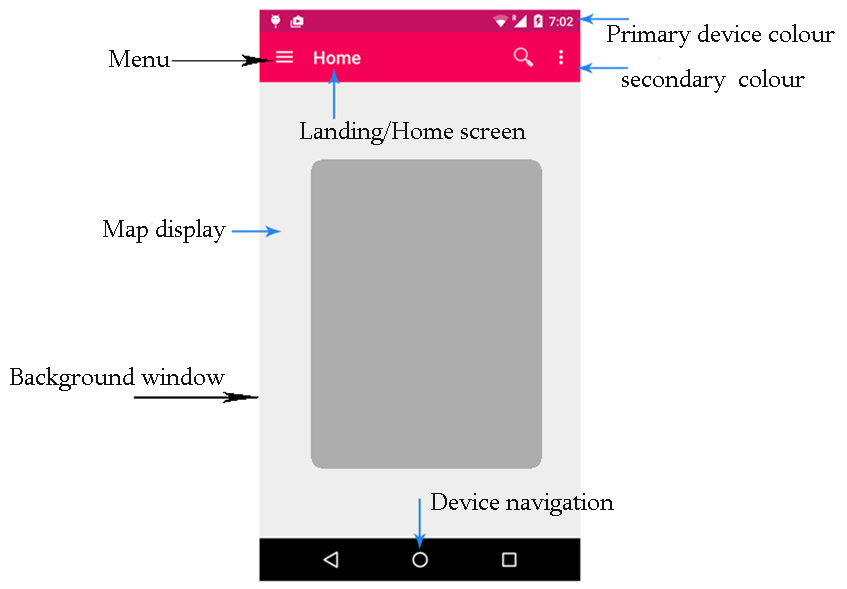
\includegraphics[width=0.5\linewidth]{Images/userInterface.jpg}\\[0.5cm]
				
	\subsubsection{Hardware Interfaces}
				The NavUp hardware interface will primarily be dependant on the User’s unique device. Either a Tablet, mobile phone, phablet. 	
					
	\subsubsection{Software Interfaces}
				The NavUp software  interface will primarily be dependant on the Users device and operating system of that device (IOS, Android , Windows phone). But the general layout for android operating system is depicted in the image bellow:
				
				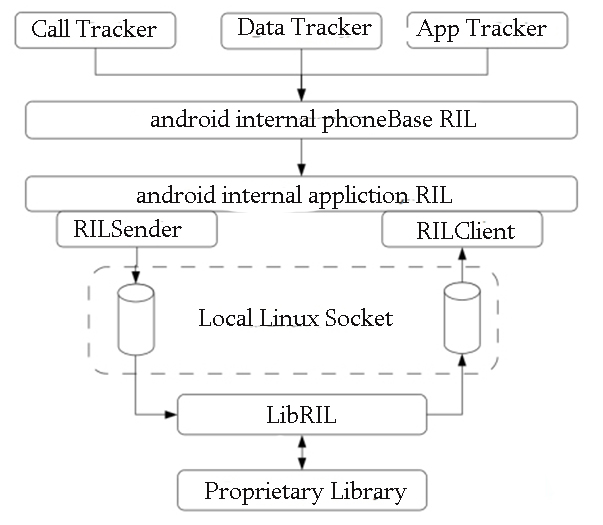
\includegraphics[width=0.5\linewidth]{Images/software.jpg}\\[0.5cm]
						
		\subsection{Functional Requirements:}
		
		\subsection{Functional Requirements:}
		
		\subsubsection{Functional Requirements List:}
		
		\begin{itemize}
			\item FR1. User Registration - The system should allow the user to create an account using their email and a password. They should also have an option to sign in through another social media account.
			
			\item FR2. User Login - Given that the user was able to register the system should allow the user to login. After the first login the system should automatically log the user in.
			
			\item FR3. User Profile - The system should allow the user to CRUD their profile.
			
			\item FR4. User Password - If the user forgets their password the system should allow them to reset it. To reset their password there should be a security check or validation.
			
			\item FR5. Search - The system should allow the user should be able to search for locations, points of interest and events. The user should also be able to specify the type of location he is searching for, like restaurants or lecture halls.
			
			\item FR6. - Current Location - The system should provide the user with their current location. The system should also allow the user to share their current location with another user.
			
			\item FR7. Navigation to Location - The system should allow the user to select a location on the map or from the search results. Once the user has selected a location a route should be calculated based on the user's preferences. The user should then be navigated turn-by-turn to their destination. The user should also be given the directions in a list. If the user locks their phone the directions should be pushed as notifications.
			
			\item FR8. Heat Maps - The system should display a heat map of campus. While navigating this heat map should continuously be updated. The heat map data should be calculated based on the number of devices connected to Wi-Fi connection points. Data should also be collected via crowdsourcing. 
			
			\item FR9. Location Information - The system should show the user information of their current location. This information could include history of a building, significance of a point of interest. If there are any activities taking place at that location in the near future the user should be able to see this as well. The system should allow higher level users should be able to CRUD location information. The system should also save a user's favourite locations.
			
			\item FR10. Location Based Notification - The system should push notifications to users based on their current location. The notification should be given based on the user's interests. The user should also have an option to block notifications for certain locations. 
			
			\item FR11. Activities Rewards - The system should keep track of rewards. When a user completes an activity specified by a third party user, the user should be notified that they successfully completed the activity and that they are eligible to receive a reward. The system must also notify the third party who created the reward who has won it.
			
			\item FR12. Active Rewards - The system should keep track of the user's steps. The user should be rewarded with virtual badges for completing active activities. These virtual badges could be rewarded for the most number steps taken in a week the highest average steps taken in a week. The user should be able to view how far they are from receiving these badges.
			
			\item FR13. Events - The system should allow for third party users to create special events that users can participate in. These events include competitions, specials at stores and restaurants, and social events. 
		\end{itemize}
		
		\subsubsection{List of Use Cases:}
		
		\begin{itemize}
			\item UC1. Search for Locations - The user enters a search query to search for a location.
			\item UC2. Search for Locations with a filter - The user chooses a filter then enters his search query.
			\item UC3. Show Current Location - The user should be shown their current location on a map.
			\item UC4. Share Location - The user should be able to share their location with another user.
			\item UC5. Calculate Route Without Traffic - The user should be able to specify for their route to be calculated without traffic.
			\item UC6. Calculate Quickest Route - The user should be able to specify their route to be the quickest possible route.
			\item UC7. Navigate to Destination - The user should be given navigation instructions to get to their location.
			\item UC8. Save Location as Favourite - The user should be able to save their current or a searched location as their favourite.
			\item UC9. Show Favourites - The User should be shown a list of their favourite places.
			\item UC10. Registration - When the user opens the app he should be given the choice to register if he wants to.
			\item UC11. Login - If the user has a account the system should allow the user to login.
			\item UC12. Reopen Application after closing - The application must auto-login the user. It should also continue navigation if there was a navigation in progress.
			\item UC13. Navigate when application is closed - If the application is still open in the background the user will receive push notifications for directions.
			\item UC14. Password Reset - The user forgets their password and submits a reset request.
			\item UC15. Show Traffic - If the user has enabled heat maps the user will be shown a heat map of campus on the map.
			\item UC16. User walks past location he will be interested in - The user must receive a notification that they might be interested in this location.
			\item UC17. Block Notification - The user has the option to permanently block a notifications from a location when he gets a notification from that location.
			\item UC18. View Location Information - The user opens a location’s information page. The location’s information will be displayed on this page.
			\item UC19. CRUD Location Information - Higher level users will have access to CRUD locations.
			\item UC20. User Gets Reward - The user completes an activity which makes him eligible for a reward. The user receives a notification informing them that they have received a reward. System notifies the third party who is giving the reward.
			\item UC21. User Walks Required Steps - The user receives a notification informing them that they have achieved a goal and that they have received a badge for it.
			\item UC22. CRUD Events - A third party users have access to CRUD special events that users will be interested in.
			\item UC23. Create New Event - Third party user creates new special event. Users that might be interested will be notified immediately.
		\end{itemize}
		
		\subsubsection{Use Case Diagrams}
		Refer to next page for use case diagrams
		\begin{figure}[p]
			\vspace*{-2.7cm}
			\centering
			\makebox[\linewidth]
			{
				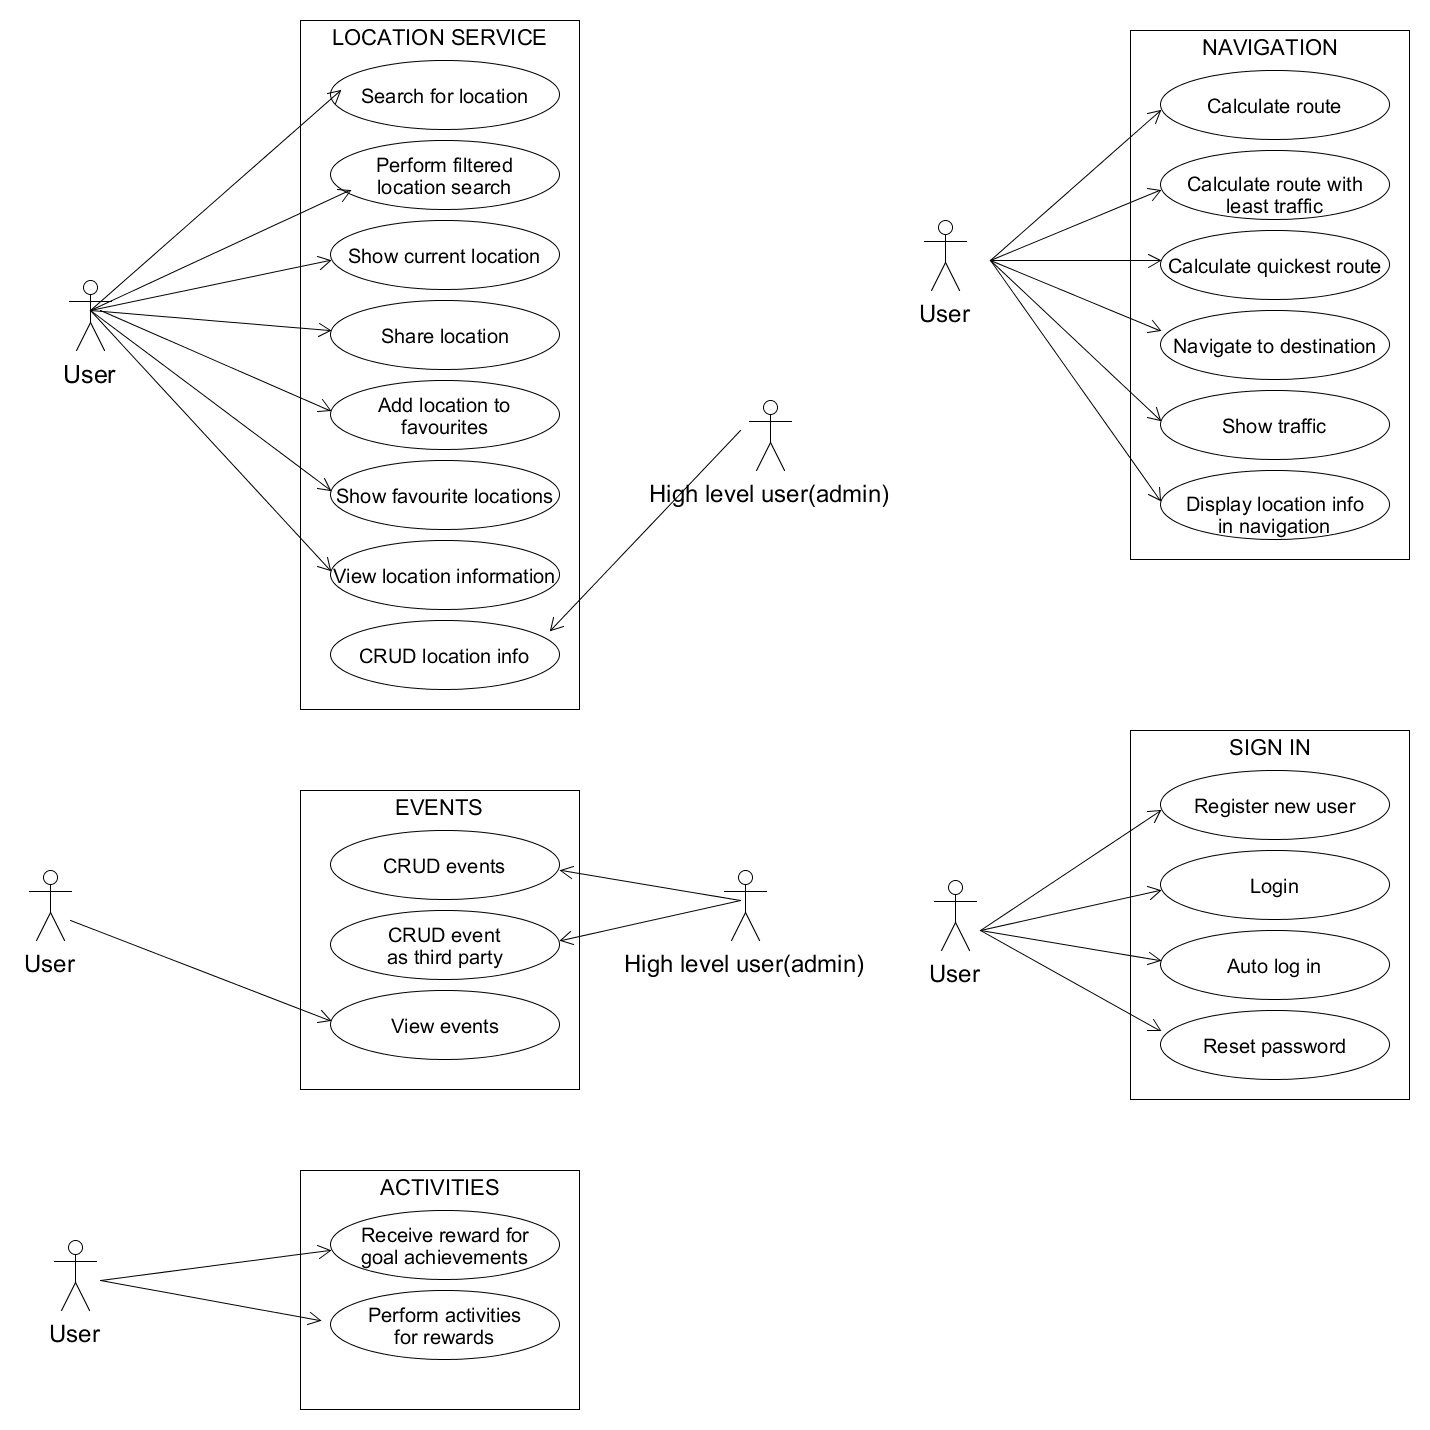
\includegraphics[width=200mm, scale=0.5]{Images/useCaseDiagrams.png}
			}\\[2cm]
			\caption{Use case diagram}
		\end{figure} 
		
		\subsubsection{Actor system interaction}
		\begin{table}[ht!]
			\centering
			\resizebox{\textwidth}{!}{%
				\begin{tabular}{|l|l|}
					\hline
					UC11:Login                          &                           \\ \hline
					Actor: User & System: App           & System : Login Service            \\ \hline
					& App displays home page    \\ \hline
					If user clicks login link           & App displays login page.  \\ \hline
					If user clicks continue link without logging in     & TUCCW navigation. \\ \hline
					TUCEW user sees welcome page        &                            \\ \hline
				\end{tabular}%
			}
		\end{table}
		
		\begin{table}[ht!]
			\centering
			\resizebox{\textwidth}{!}{%
				\begin{tabular}{|l|l|}
					\hline
					UC1:Search for locations    &                                     \\ \hline
					Actor: User                 & System: Location service            \\ \hline
					& Location service displays map with the following options \\ \hline
					TUCBW user either signs in or 
					continues without signing in   & App displays map with the following options    \\ \hline
					& Search for location. \\ \hline
					& Perform filtered search for location \\ \hline
					& Show current location \\ \hline
					& Share location \\ \hline
					& Add location to favourites \\ \hline
					& Show favourite locations \\ \hline
					& View location details \\ \hline
					
					TUCEW one of the following cases
					UC1. Search for location.                                & \\ \hline
					UC2. Perform filtered search for location                & \\ \hline
					UC3. Show current location                               & \\ \hline
					UC4. Share location                                      & \\ \hline
					UC8. Add location to favourites                          & \\ \hline
					UC9. Show favourite locations                            & \\ \hline
					UC18. View location details                               & \\ \hline
				\end{tabular}%
			}
		\end{table}
		
		\begin{table}[ht!]
			\centering
			\resizebox{\textwidth}{!}{%
				\begin{tabular}{|l|l|}
					\hline
					UC7:Navigate to destination    &                                     \\ \hline
					Actor: User                 & System: Navigation            \\ \hline
					& Navigation displays navigation page with the following options \\ \hline
					TUCBW User sees navigation page   &                         \\ \hline
					& Calculate route without traffic.    \\ \hline
					& Calculate quickest route \\ \hline
					
					TUCEW one of the following cases
					UC5.Calculate route without traffic. &    \\ \hline
					UC6.Calculate quickest route.        &    \\ \hline
				\end{tabular}%
			}
		\end{table}
		
		\begin{table}[ht!]
			\centering
			\resizebox{\textwidth}{!}{%
				\begin{tabular}{|l|l|}
					\hline
					UC5:Calculate route without traffic    &                          \\ \hline
					Actor: User                 &           System: Navigation        \\ \hline
					&       User has selected destination \\ \hline
					TUCBW User clicks "Calculate route" button after selecting destination &                                      \\ \hline
					& App displays home page              \\ \hline
					If user clicks calculate route without traffic button & App determines and displays route on map with least traffic.            \\ \hline \hline
				\end{tabular}%
			}
		\end{table}
		
		\begin{table}[ht!]
			\centering
			\resizebox{\textwidth}{!}{%
				\begin{tabular}{|l|l|}
					\hline
					UC6:Calculate quickest route    &                                     \\ \hline
					Actor: User                 &       System: Navigation               \\ \hline
					&       User has selected destination \\ \hline
					TUCBW User clicks "Calculate route" button after selecting destination & \\ \hline
					& App displays home page              \\ \hline
					If user clicks calculate quickest route button & App determines and displays quickest route.            \\ \hline \hline
				\end{tabular}%
			}
		\end{table}
		
		\begin{table}[ht!]
			\centering
			\resizebox{\textwidth}{!}{%
				\begin{tabular}{|l|l|}
					\hline
					UC3:Show current location   &                                      \\ \hline
					Actor: User                 &           System: Location service   \\ \hline
					&           Map has finished loading \\ \hline
					TUCBW user clicks "show current location" button & Location service determines user location\\ \hline
					&           User location and data shown on map     \\ \hline
					\\ \hline
				\end{tabular}%
			}
		\end{table}
		
		\begin{table}[ht!]
			\centering
			\resizebox{\textwidth}{!}{%
				\begin{tabular}{|l|l|}
					\hline
					UC4:Share location    &                                     \\ \hline
					Actor: User                 & System: Location service  \\ \hline
					& User is at/selects point of interest \\ \hline
					TUCBW                       &                                      \\ \hline
					If user clicks share button & App shares current location with other app users. \\ \hline \hline
				\end{tabular}%
			}
		\end{table}
		
		\begin{table}[ht!]
			\centering
			\resizebox{\textwidth}{!}{%
				\begin{tabular}{|l|l|}
					\hline
					UC2:Perform filtered search for location    &                     \\ \hline
					Actor: User                 & System: Location service            \\ \hline
					TUCBW search bar is clicked & Filter options are displayed        \\ \hline
					
					If user clicks on filter button   & App performs search based on filters chosen by user. \\ \hline
					TUCEW user sees search results & \\ \hline
				\end{tabular}%
			}
		\end{table}
		
		\begin{table}[ht!]
			\centering
			\resizebox{\textwidth}{!}{%
				\begin{tabular}{|l|l|}
					\hline
					UC8:Save location to favourites    &                                     \\ \hline
					Actor: User                 &           System: Location service               \\ \hline
					& User is at/selects point of interest \\ \hline
					TUCBW "Save location button is pressed" &                          \\ \hline
					If user clicks save location button   & App adds location to list  \\ \hline
					TUCEW confirmation dialog appears           &                           \\ \hline
					& updated favourites list displayed \\ \hline
				\end{tabular}%
			}
		\end{table}
		
		\begin{table}[ht!]
			\centering
			\resizebox{\textwidth}{!}{%
				\begin{tabular}{|l|l|}
					\hline
					UC9:Show favourites   			&                                     \\ \hline
					Actor: User                 		&           System: Location Service       \\ \hline
					TUCBW "Show favourites button is clicked" & App fetches list of favourites from server \\ \hline
					TUCEW favourites page displayed          &                              \\ \hline
				\end{tabular}%
			}
		\end{table}
		
		
		
		
		\begin{table}[ht!]
			\centering
			\resizebox{\textwidth}{!}{%
				\begin{tabular}{|l|l|}
					\hline
					UC10:Registration    &                                     \\ \hline
					Actor: User                 &           System: Login               \\ \hline
					TUCBW                       &                                      \\ \hline
					& App displays home page              \\ \hline
					If user clicks login link   & App displays login page.            \\ \hline
					If user clicks continue link without logging in & TUCCW navigation. \\ \hline
					TUCEW user sees home page          &                              \\ \hline
					& User directed to home page
				\end{tabular}%
			}
		\end{table}
		
		\begin{table}[ht!]
			\centering
			\resizebox{\textwidth}{!}{%
				\begin{tabular}{|l|l|}
					\hline
					UC12:Reopen app after closing    &                                   \\ \hline
					Actor: User                 &           System: App               \\ \hline
					& App currently minimized/in use\\ \hline
					TUCBW App is reopened       & User signed in automatically  \\ \hline
					& App displays home page              \\ \hline
					TUCEW user sees home page   &                              \\ \hline
				\end{tabular}%
			}
		\end{table}	\
		
		\begin{table}[ht!]
			\centering
			\resizebox{\textwidth}{!}{%
				\begin{tabular}{|l|l|}
					\hline
					UC13:Navigation when app is closed    &                                     \\ \hline
					Actor: User                	 &           System: Navigation               \\ \hline
					&           App running in background\\ \hline
					TUCBW app minimized while navigation in process & \\ \hline
					TUCEW app is reopened/arrival at destination                      &                              \\ \hline
				\end{tabular}%
			}
		\end{table}
		
		\begin{table}[ht!]
			\centering
			\resizebox{\textwidth}{!}{%
				\begin{tabular}{|l|l|}
					\hline
					UC14:Password reset    			   &                                     \\ \hline
					Actor: User                		   & System: Login               \\ \hline
					TUCBW User clicks "forgot password" button & App displays password retrieval page   \\ \hline
					& App displays home page              \\ \hline
					TUCEW user sees welcome page         	   &                           \\ \hline
				\end{tabular}%
			}
		\end{table}
		
		\begin{table}[ht!]
			\centering
			\resizebox{\textwidth}{!}{%
				\begin{tabular}{|l|l|}
					\hline
					UC15:Show traffic    			&                                     \\ \hline
					Actor: User                 		&           System: Navigation               \\ \hline
					& Map already loaded \\ \hline
					TUCBW "Show traffic option is selected" & fetch traffc data and display as heat map\\ \hline
					TUCEW user sees traffic data on map      &                              \\ \hline
				\end{tabular}%
			}
		\end{table}
		
		\begin{table}[ht!]
			\centering
			\resizebox{\textwidth}{!}{%
				\begin{tabular}{|l|l|}
					\hline
					UC16:User walks past location he will be interested in    &                                     \\ \hline
					Actor: User                 &           System: App               \\ \hline
					TUCBW User walking past point of interest & App displays location \\ \hline
					TUCEW User walking away from point of interest & \\ \hline
				\end{tabular}%
			}
		\end{table}
		
		\begin{table}[ht!]
			\centering
			\resizebox{\textwidth}{!}{%
				\begin{tabular}{|l|l|}
					\hline
					UC17:Block notifications    &                                     \\ \hline
					Actor: User                 &  System: Notification               \\ \hline
					& User receives notification \\ \hline
					TUCBW User selects "block notifications" option & App dismisses notification\\ \hline
					TUCEW Particular location added to "blocked" list &                              \\ \hline
				\end{tabular}%
			}
		\end{table}
		
		\begin{table}[ht!]
			\centering
			\resizebox{\textwidth}{!}{%
				\begin{tabular}{|l|l|}
					\hline
					UC18:View location information    &                                     \\ \hline
					Actor: User                 &           System: App               \\ \hline
					TUCBW user clicks location information link &  \\ \hline
					TUCEW Location information displayed on screen          &                              \\ \hline
				\end{tabular}%
			}
		\end{table}
		
		\begin{table}[ht!]
			\centering
			\resizebox{\textwidth}{!}{%
				\begin{tabular}{|l|l|}
					\hline
					UC19:CRUD location information    &                                     \\ \hline
					Actor: High level user                 & System: App               \\ \hline
					& Display location information management page \\ \hline
					TUCBW  Location information management page is loaded &                                      \\ \hline
					TUCEW High level user CRUD location information  &                              \\ \hline
				\end{tabular}%
			}
		\end{table}
		
		\begin{table}[ht!]
			\centering
			\resizebox{\textwidth}{!}{%
				\begin{tabular}{|l|l|}
					\hline
					UC20:User gets reward    &                                     \\ \hline
					Actor: User                 &           System: Activities               \\ \hline
					TUCBW User achieves set goal eligible for reward & System grants user eligibility to collect reward\\ \hline
					TUCEW user collects reward/waits to collect later          &                              \\ \hline
				\end{tabular}%
			}
		\end{table}
		
		\begin{table}[ht!]
			\centering
			\resizebox{\textwidth}{!}{%
				\begin{tabular}{|l|l|}
					\hline
					UC16:User walks required steps    &                                     \\ \hline
					Actor: User                 &           System: Activities               \\ \hline
					TUCBW User's steps walked reach set number & \\ \hline
					& App displays banner message              \\ \hline
					If user takes no action wait & App displays login page.            \\ \hline
					Click banner or open app to retrieve reward & Rewards page displayed. \\ \hline
					TUCEW banner message disappears after set time & \\ \hline
				\end{tabular}%
			}
		\end{table}
		
		\begin{table}[ht!]
			\centering
			\resizebox{\textwidth}{!}{%
				\begin{tabular}{|l|l|}
					\hline
					UC22:CRUD events    &                                     \\ \hline
					Actor: User                 &           System: App               \\ \hline
					& Event management page diaplayed \\ \hline
					TUCBW Third party user sees events management page & \\ \hline
					TUCEW Third party user CRUD events  & \\ \hline
				\end{tabular}%
			}
		\end{table}
		
		\begin{table}[ht!]
			\centering
			\resizebox{\textwidth}{!}{%
				\begin{tabular}{|l|l|}
					\hline
					UC23:Create event as third party   	&                                     \\ \hline
					Actor: User                 		&           System: Events               \\ \hline
					TUCBW "Create event" button is clicked  & Page displayed to capture details  \\ \hline
					TUCEW Event added to location details         	 &                              \\ \hline
				\end{tabular}%
			}
		\end{table}
		
		
		\begin{landscape}
			\subsubsection{Traceability Matrix}
			\begin{table}[ht!]
				\centering
				\resizebox{\textwidth}{!}{%
					\begin{tabular}{|c|c|c|c|c|c|c|c|c|c|c|c|c|c|c|c|c|c|c|c|c|c|c|c|c|}
						\hline
						Requirement           & Priority           & UC1        & UC2        & UC3        & UC4        & UC5        & UC6        & UC7        & UC8        & UC9        & UC10       & UC11       & UC12       & UC13       & UC14       & UC15       & UC16       & UC17       & UC18       & UC19       & UC20       & UC21       & UC22       & UC23       \\ \hline
						FR1                   & 3                  &            &            &            &            &            &            &            &            &            & X          &            &            &            &            &            &            &            &            &            &            &            &            &            \\ \hline
						\textbf{FR2}          & \textbf{3}         & \textbf{}  & \textbf{}  & \textbf{}  & \textbf{}  & \textbf{}  & \textbf{}  & \textbf{}  & \textbf{}  & \textbf{}  & \textbf{}  & \textbf{X} & \textbf{X} & \textbf{}  & \textbf{}  & \textbf{}  & \textbf{}  & \textbf{}  & \textbf{}  & \textbf{}  & \textbf{}  & \textbf{}  & \textbf{X} & \textbf{X} \\ \hline
						\textbf{FR3}          & \textbf{3}         & \textbf{}  & \textbf{}  & \textbf{}  & \textbf{}  & \textbf{}  & \textbf{}  & \textbf{}  & \textbf{X} & \textbf{X} & \textbf{X} & \textbf{X} & \textbf{}  & \textbf{}  & \textbf{X} & \textbf{}  & \textbf{}  & \textbf{}  & \textbf{}  & \textbf{}  & \textbf{}  & \textbf{}  & \textbf{}  & \textbf{}  \\ \hline
						\textbf{FR4}          & \textbf{3}         & \textbf{}  & \textbf{}  & \textbf{}  & \textbf{}  & \textbf{}  & \textbf{}  & \textbf{}  & \textbf{}  & \textbf{}  & \textbf{}  & \textbf{}  & \textbf{}  & \textbf{}  & \textbf{X} & \textbf{}  & \textbf{}  & \textbf{}  & \textbf{}  & \textbf{}  & \textbf{}  & \textbf{}  & \textbf{}  & \textbf{}  \\ \hline
						\textbf{FR5}          & \textbf{5}         & \textbf{X} & \textbf{X} & \textbf{}  & \textbf{}  & \textbf{}  & \textbf{}  & \textbf{}  & \textbf{}  & \textbf{}  & \textbf{}  & \textbf{}  & \textbf{}  & \textbf{}  & \textbf{}  & \textbf{}  & \textbf{}  & \textbf{}  & \textbf{}  & \textbf{}  & \textbf{}  & \textbf{}  & \textbf{}  & \textbf{}  \\ \hline
						\textbf{FR6}          & \textbf{6}         & \textbf{}  & \textbf{}  & \textbf{X} & \textbf{X} & \textbf{}  & \textbf{}  & \textbf{}  & \textbf{X} & \textbf{}  & \textbf{}  & \textbf{}  & \textbf{}  & \textbf{}  & \textbf{}  & \textbf{}  & \textbf{X} & \textbf{}  & \textbf{X} & \textbf{}  & \textbf{}  & \textbf{}  & \textbf{}  & \textbf{}  \\ \hline
						\textbf{FR7}          & \textbf{6}         & \textbf{}  & \textbf{}  & \textbf{}  & \textbf{}  & \textbf{X} & \textbf{X} & \textbf{X} & \textbf{}  & \textbf{}  & \textbf{}  & \textbf{}  & \textbf{X} & \textbf{X} & \textbf{}  & \textbf{}  & \textbf{}  & \textbf{}  & \textbf{}  & \textbf{}  & \textbf{}  & \textbf{}  & \textbf{}  & \textbf{}  \\ \hline
						\textbf{FR8}          & \textbf{4}         & \textbf{}  & \textbf{}  & \textbf{}  & \textbf{}  & \textbf{X} & \textbf{}  & \textbf{}  & \textbf{}  & \textbf{}  & \textbf{}  & \textbf{}  & \textbf{}  & \textbf{}  & \textbf{}  & \textbf{X} & \textbf{}  & \textbf{}  & \textbf{}  & \textbf{}  & \textbf{}  & \textbf{}  & \textbf{}  & \textbf{}  \\ \hline
						\textbf{FR9}          & \textbf{5}         & \textbf{}  & \textbf{}  & \textbf{}  & \textbf{}  & \textbf{}  & \textbf{}  & \textbf{}  & \textbf{}  & \textbf{X} & \textbf{}  & \textbf{}  & \textbf{}  & \textbf{}  & \textbf{}  & \textbf{}  & \textbf{}  & \textbf{}  & \textbf{}  & \textbf{X} & \textbf{X} & \textbf{}  & \textbf{}  & \textbf{}  \\ \hline
						\textbf{FR10}         & \textbf{4}         & \textbf{}  & \textbf{}  & \textbf{}  & \textbf{}  & \textbf{}  & \textbf{}  & \textbf{}  & \textbf{}  & \textbf{}  & \textbf{}  & \textbf{}  & \textbf{}  & \textbf{}  & \textbf{}  & \textbf{}  & \textbf{X} & \textbf{X} & \textbf{}  & \textbf{}  & \textbf{}  & \textbf{}  & \textbf{}  & \textbf{}  \\ \hline
						\textbf{FR11}         & \textbf{3}         & \textbf{}  & \textbf{}  & \textbf{}  & \textbf{}  & \textbf{}  & \textbf{}  & \textbf{}  & \textbf{}  & \textbf{}  & \textbf{}  & \textbf{}  & \textbf{}  & \textbf{}  & \textbf{}  & \textbf{}  & \textbf{}  & \textbf{}  & \textbf{}  & \textbf{}  & \textbf{X} & \textbf{}  & \textbf{}  & \textbf{}  \\ \hline
						\textbf{FR12}         & \textbf{1}         & \textbf{}  & \textbf{}  & \textbf{}  & \textbf{}  & \textbf{}  & \textbf{}  & \textbf{}  & \textbf{}  & \textbf{}  & \textbf{}  & \textbf{}  & \textbf{}  & \textbf{}  & \textbf{}  & \textbf{}  & \textbf{}  & \textbf{}  & \textbf{}  & \textbf{}  & \textbf{}  & \textbf{X} & \textbf{}  & \textbf{}  \\ \hline
						\textbf{FR13}         & \textbf{3}         & \textbf{}  & \textbf{}  & \textbf{}  & \textbf{}  & \textbf{}  & \textbf{}  & \textbf{}  & \textbf{}  & \textbf{}  & \textbf{}  & \textbf{}  & \textbf{}  & \textbf{}  & \textbf{}  & \textbf{}  & \textbf{}  & \textbf{}  & \textbf{}  & \textbf{}  & \textbf{}  & \textbf{}  & \textbf{X} & \textbf{X} \\ \hline
						\multicolumn{2}{|c|}{\textbf{UC Priority}} & \textbf{5} & \textbf{5} & \textbf{6} & \textbf{3} & \textbf{5} & \textbf{5} & \textbf{5} & \textbf{6} & \textbf{3} & \textbf{3} & \textbf{4} & \textbf{3} & \textbf{3} & \textbf{4} & \textbf{5} & \textbf{4} & \textbf{2} & \textbf{6} & \textbf{6} & \textbf{3} & \textbf{2} & \textbf{4} & \textbf{4} \\ \hline
					\end{tabular}%
				}
			\end{table}
		\end{landscape}
		

		\subsection{Performance Requirements}
			\begin{enumerate}
				\item Low battery consumption
					\begin{itemize}
						\item Since the application uses predominantly Wifi will be priority to minimize impact on the battery of the phone since battery life is high concern of the users.   
						\item Numerous calls to various functions when navigating the user from point A to point B, thus optimising this functionality will be a great concern since this can become a high impact on the battery, draining it rather fast.
						\item With the added assumption that the user will grant permission to allow us transmit the device's location in attempt to help the application to navigate the user to locations with no signal for GPS but have WiFi accessibility.
						\item Heat map generation will require additional request sent from devices to the routers if this is constantly updated it will start impacting the battery heavily.
					\end{itemize}
				\item Fast real-time navigation updates
					\begin{itemize}
						\item Important aspect of navigating a user is the accuracy of the process. Thus making use of available resource effectively can create an accurate representation and navigation the user to the desired location. The resources that will be used is the Heat Map, other user locations, WiFi and GPS when available.
					\end{itemize}
				\item Accurate Step Counting
					\begin{itemize}
						\item Awards will be awarded based on steps taken thus the counting must use as much of the resources at its deposal to be as accurate as possible to distinguish between actual walking and people bouncing their legs when seated or swinging their phone around to attempt to fool the system.
					\end{itemize}
				\item Accurate location tracking
					\begin{itemize}
						\item This is the main promise of the application. Everything will be off and wrong if the location is inaccurate. Thus this performance requirement will be most important.
					\end{itemize}  
			\end{enumerate}
      
		\subsection{Design Constraints}
    		The database has to be able to handle more than 30000 users. The applications is supposed to be designed in such a way 			that it can work with WiFi, GPS and Mobile networks. It should switch between WiFi as necessary.

		    The application will need hard drive space on the device. The lack thereof will result in an inability to download. 			Based on research the application should need between 100 - 200 MB of harddrive space. 

		    Memory usage will be high because the application will always be running in order to track the user’s steps unless the 			user decides otherwise. The data should not be more than 20MB.

		\subsection{Software System Attributes}
			\begin{enumerate}
				\item Reliability 
					\begin{itemize}
						\item Our system makes a lot of assumptions in terms of certain resources that will be available along with permission to use them. Such as User permission to access their GPS/Location/WiFi/Accelerometer.
						\item Our system relies on availability of WiFi accros the campus of the University of Pretoria, that campus has power and or the generators work if there is no power.
					\end{itemize}
				\item Security 
					\begin{itemize}
						\item There are four levels of Users with each having similar and different rights. The differences must be sure to authenticate the user trying to execute the function. If the user is not authorised to do so they must be denied access or if they are authorised they must be allowed to continue.
					\end{itemize}
				\item Availability
					\begin{itemize}
						\item The avaibility is non existant if the user denies all of the permissions. If we do not have access to the device's GPS/Location/WiFi/Accelerometer none of the application's functionality will be able to work.
						\item Limited availability overall but the main functionality will be achieved with permission to use the user's Location and the user's WiFi.
						\item Most accurate functionality of the main functions can be achieved with permission to use Location/WiFi and GPS of the device and use the user's permission to send anonmous pings to generate heat maps and use other devices' location to navigate the user.
					\end{itemize}
			\end{enumerate}
	
\end{document}
